%!TEX root = ../Thesis.tex


\section{Projekt-Architektur}\label{Projekt-Architektur}
Die Ordnerstruktur des Projekts ist in \autoref{fig:dir_struc_root} zu sehen.
Die Strukturen für das Frontend, Backend sowie den NodeMCU Code sind in \autoref{anh:Projekt-Architektur} zu finden.

\begin{figure}[H]
    \centering
    \begin{minipage}[t]{1\textwidth}
        \caption{Root-Ordnerstruktur}
        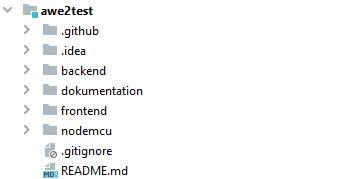
\includegraphics[width=0.5\textwidth]{img/dir_struc_root.png}\\
        \source{Eigene Darstellung}
        \label{fig:dir_struc_root}
    \end{minipage}
\end{figure}

Die Quelltexte der drei Komponenten NodeMCU, Backend und Frontend sind voneinander getrennt, werden aber als ein Gesamtprojekt ausgeliefert.

\subsection{Frontend}
Die Struktur des Frontend-Quellcodes ist eine Mischung aus klassicher Web- und Nodejs- Projektstruktur.
In dem Ordner \textit{resources} sind Ressourcen zu finden, welche der Webserver den Clients bereitstellt.
Diese sind in \textit{css}, \textit{img} und \textit{js} gegliedert.
Verwendete Libraries, wie z.B. \textit{sir.js} befinden sich in eigenen Unterordnern, während der eigenentwickelte
Quellcode sich direkt in den Ordnern befindet.

Im Root-Ordner des Frontends befinden sich ,für die Komponente, globale Dateien, wie z.B. das Buildscript für Docker,
die \textit{package.json} für Node.js und die \textit{.eslintrc.json} zur Konfiguration des JavaScript-Linters.

\subsection{Backend}
Die Struktur das Backend-Quellcodes orientiert sich an der üblichen Struktur für Node.js Projekte, ist jedoch
absichtlich simpel und flach, anstatt tief hierarchisch, gestaltet.
Dies ermöglicht bei der kleinen Größe der Anwendung eine effizientere Navigation durch die Dateien.
In dem Unterordner \textit{src} befinden die Quelltexte des Backends, in \textit{test} die Quelltextdatei testMain.js
sowie die testData.js, welche nur zum Generieren von Testdaten verwendet wird.
\subsection{NodeMCU}
In dieser Komponente befindet sich im Unterordner \textit{src/nocemcu} die aktuell einzige Quelltextdatei für den NodeMCU.
Im Ordner \textit{ress} befindet sich zusätzlich eine Tabelle des Wirings von dem NodeMCU und dem BME280-Sensor.





